

%For demonstration, we modeled a UAV system. The target application is waterway monitor. The waterway area consists of a set of fly-in zones and fly-out zones. The goal of the UAV is to fly from one end of the waterway to the other end in minimum distance, while staying inside the fly-in zones and outside the fly-out zones.
 
The CASE toolchain was developed as a part of the DARPA CASE program to help system engineers design cyber-physical systems that satisfy cyber-resiliency requirements.
A UAV surveillance system was modeled as a part of the demonstration effort,
and the UAV's goal was to fly from one end of a (meandering) waterway to the other while adhering to a set of keep-in and keep-out zones.

Figure~\ref{SW} shows an overview of the software architecture.
The baseline UAV software contained the UxAS~\cite{uxas} flight planning component, waypoint plan manager, UART driver, radio driver, and fly-zone database.
These components were associated with varying levels of trustworthiness.
In particular, UxAS was treated as blackbox software and deemed as potentially security-compromised since it was an open-source component developed by a third party.
The CASE cyber-security analysis tools generated a list of requirements for mitigating cyber-security vulnerabilities detected in the UAV model,
and these requirements were addressed using the CASE model transformation tools.
The transformations inserted eight high-assurance components into the model including attestation management, monitors, and filters.
%: attestation gate, attestation manager, two monitors, and four filters.
AGREE behavioral specifications for these components were provided, corresponding to their intended functionality.
%manually entered by the user based on the cyber-security vulnerabilities being mitigated.

\begin{figure}[ht!]
\centering
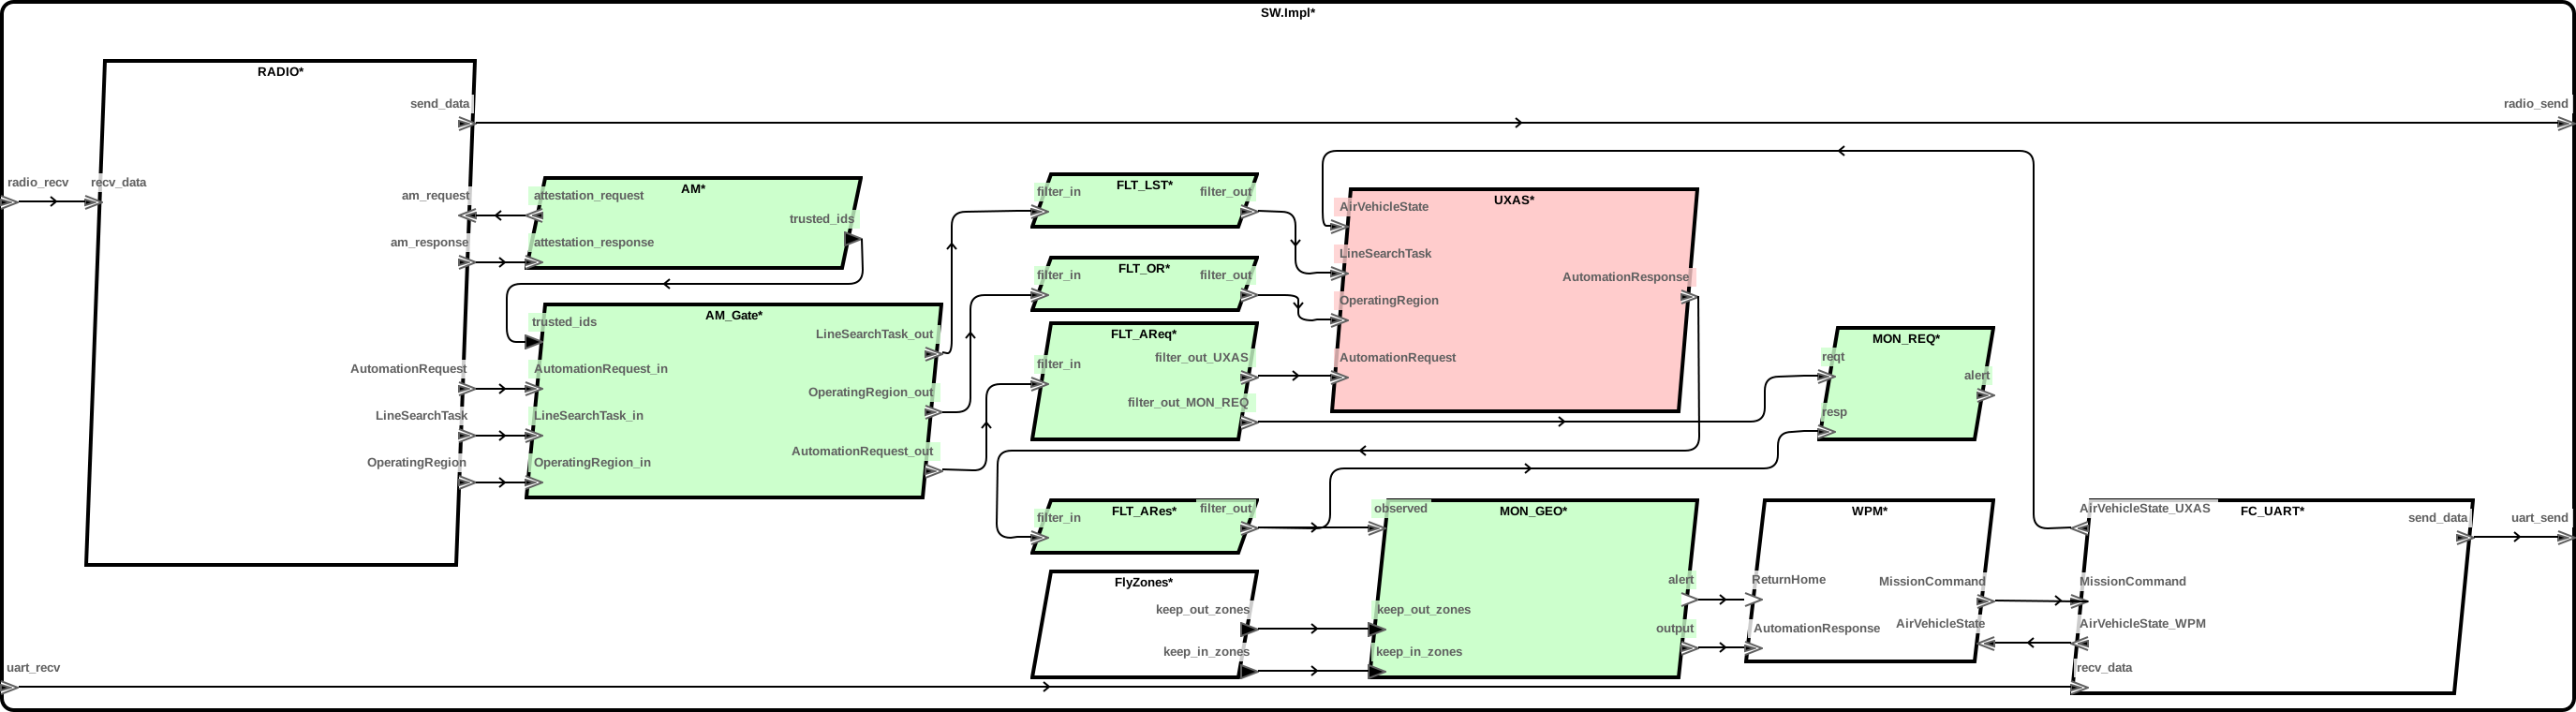
\includegraphics[width=120mm]{sw3.png}
\caption{A UAV Software Architecture Model in AADL \label{SW}}
\end{figure}

The hardened model (baseline plus high-assurance components) contained 13 threads,
all of which were mapped to a single mission computer processor running the seL4 microkernel (chosen for its formally verified separation guarantees).
An seL4 domain schedule was added to the model with all threads designated to run once per scheduling cycle with a period of 500 ms.
The processor time allocated to each thread ranged from 2 ms (filters and monitors) to 100 ms (UxAS).
The verification goal was to prove that the key system security properties were satisfied by the hardened model with the components executing according to the seL4 domain schedule.

We note that although \textit{event} and \textit{event data} ports were used in the UAV AADL model, they were intended to model the event-triggered execution of periodic threads.
In addition, since each thread executes once every scheduling cycle, the number of queued events or data is always equal to or less than one,
making this model suitable for the application of our modeling framework.

The following system-level security properties were to be verified in the presence of the seL4 domain schedule:
\begin{itemize}
	\item The output UART and RF messages are \emph{well-formed}
	\item The system only accepts commands from \emph{trusted} sources
	\item The generated waypoints fall within the boundary of a defined \emph{geo-fence}
\end{itemize}
Our framework was able to prove these properties in less than 2 minutes on a PC with 2.6 GHz CPU and 32 GB RAM.

